\documentclass[twoside, openany, 11pt]{article}
% ========== Packages ==========

\usepackage[a4paper,
  left=25mm,
  right=25mm,
  top=30mm,
  bottom=35mm,
  headheight=35mm
]{geometry}

\usepackage[ngerman]{babel} %Ändert die Sprache
\usepackage[T1]{fontenc} %Wichtig für ä ö ü
\usepackage{amssymb} %Für mathematische Zeichen
\usepackage{amsthm} %Für mathematische Umgebungen
\usepackage{graphicx}
\usepackage{fancyhdr}
\usepackage[utf8]{inputenc}
\usepackage{multirow} %Für Tabellen
\usepackage{longtable} %Für lange Tabellen
\usepackage{tabularx}
\usepackage{pdfpages} %Zum einfügen von PDF's
\usepackage{hyperref} %Für hyperlinks
\hypersetup{
    bookmarks=true,
}
\usepackage{parskip}

\usepackage{caption} %Für die Beschriftung von Bilder
\captionsetup{justification=centering}
\captionsetup{font=it}
\setlength{\parindent}{0pt}
\usepackage{subcaption} %Für die Beschriftung unterteilter Bilder
\usepackage{float}
\floatstyle{plaintop}
\restylefloat{table}

\makeatletter %Für römische Zahlen
\newcommand*{\rom}[1]{\expandafter\@slowromancap\romannumeral #1@}

%Für die dicken Linien in Tabellen
\def\thickhline{%
  \noalign{\ifnum0=`}\fi\hrule \@height \thickarrayrulewidth \futurelet
   \reserved@a\@xthickhline}
\def\@xthickhline{\ifx\reserved@a\thickhline
               \vskip\doublerulesep
               \vskip-\thickarrayrulewidth
               \fi
      \ifnum0=`{\fi}}
\makeatother

\newlength{\thickarrayrulewidth}
\setlength{\thickarrayrulewidth}{2\arrayrulewidth}
\raggedbottom %Sorgt dafür, dass nicht immer alles auf die ganze Seite verteilt wird.

%Eigens erstellte Variablen
\newcommand{\plotWidth}{0.7}
\newcommand{\garphWidth}{0.7}

% ========== Header and Footer ==========
\pagestyle{fancy}
\fancyhf{}
\fancyhead[RE,LO]{Seite \thepage}
\fancyhead[LE,RO]{\nouppercase{\leftmark}}
\fancyfoot[RE,LO]{PAIND HS2020}


\begin{document}
% ========== Titelseite ==========
  \begin{titlepage}
    \begin{center}
        % \vspace*{1cm}

        \LARGE
        Bachelor-Thesis an der Hochschule Luzern\\
        Technik \& Architektur

        \vspace{0.8cm}
        \Huge
        \textbf{Solar Butterfly - Auslegung Grundstruktur}

        \vspace{3cm}

        \begin{center}
          \makebox[\textwidth]{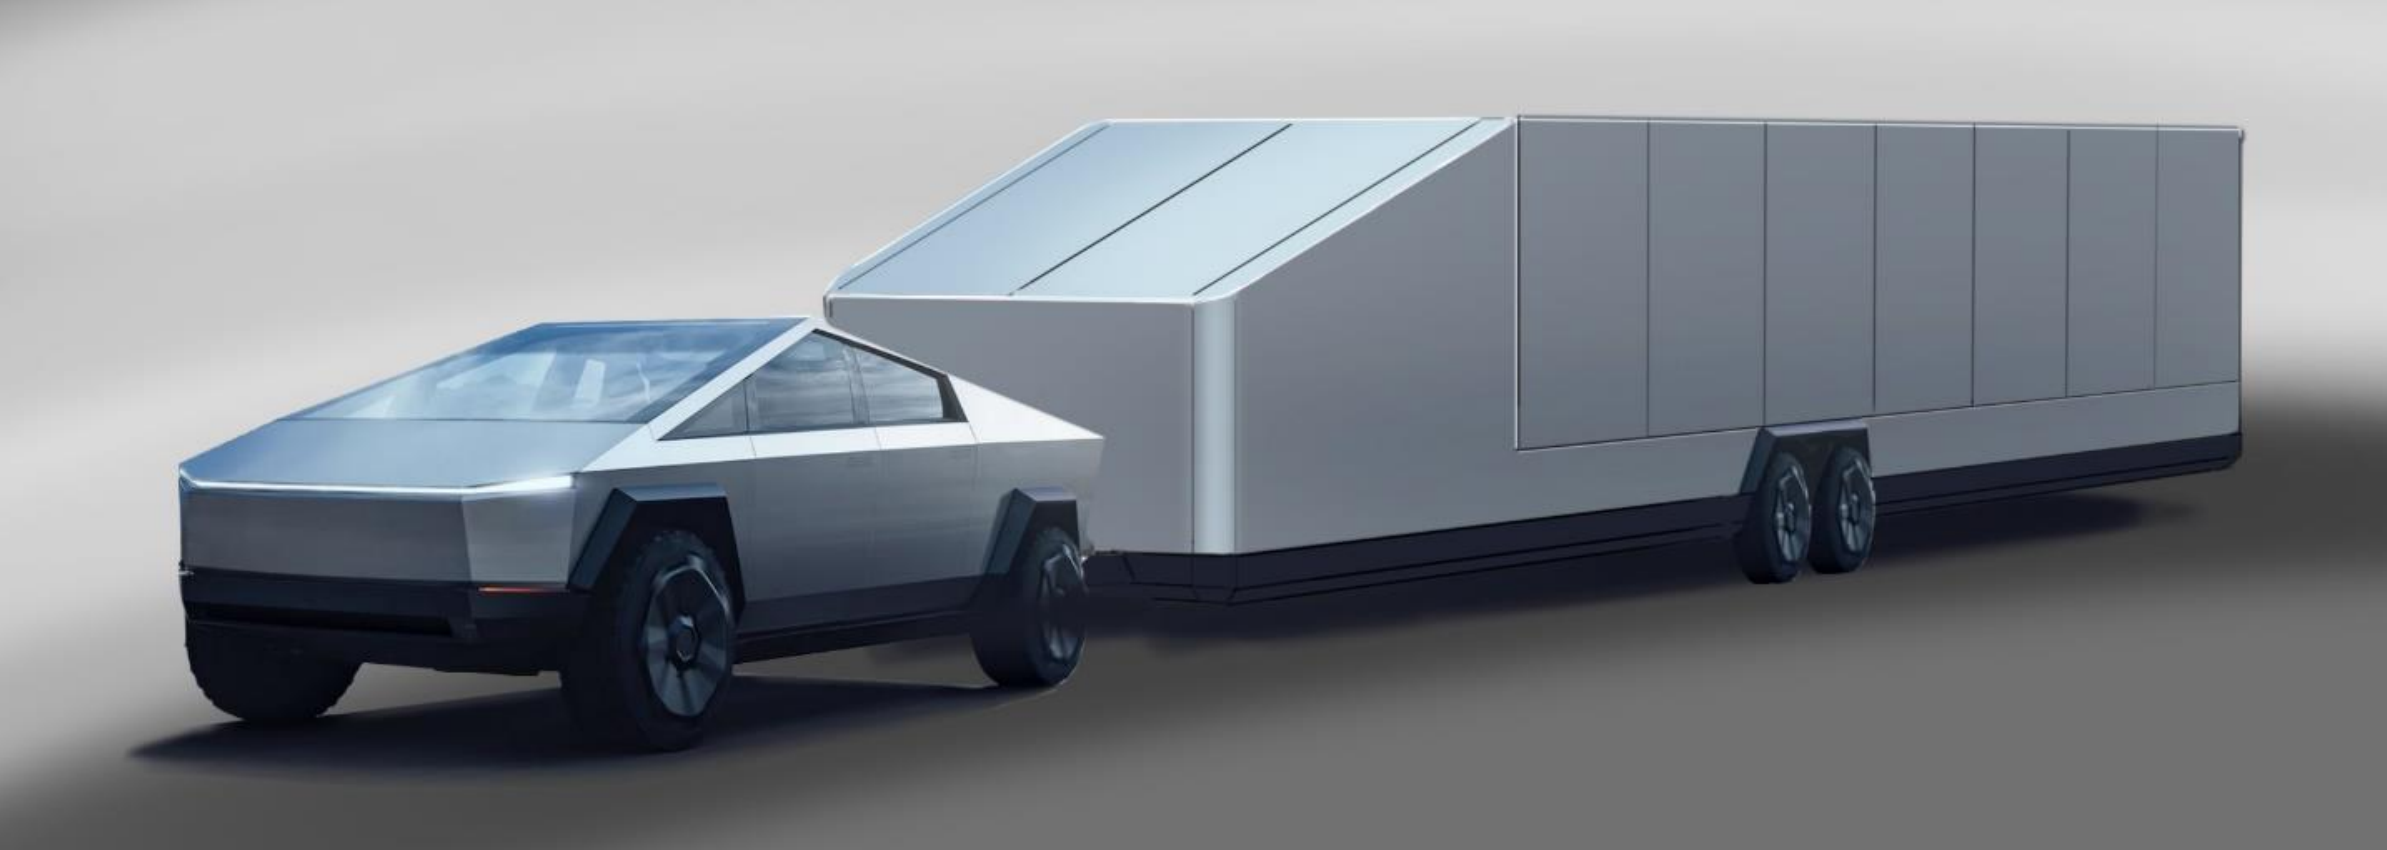
\includegraphics[width=1\paperwidth]{04_Figures/SB0.png}}
        \end{center}

        \vfill
        \begin{table}[b]
        \small
          \begin{tabularx}{\linewidth}{llX}
            \textbf{Diplomandin/Diplomand} & \textbf{Gut, Andre}                                &\\[4 mm]
            \textbf{Bachelor-Studiengang}  & \textbf{Bachelor Maschinentechnik}                 &\\[4 mm]
            \textbf{Semester}              & \textbf{FS21}                                      &\\[4 mm]
            \textbf{Dozentin/Dozent}       & \textbf{Roman\v{c}uk, Dejan}                       &\\[4 mm]
            \textbf{Expertin/Experte}      & \textbf{Dubach, Roger}                             &
          \end{tabularx}
        \end{table}

    \end{center}
\end{titlepage}


% ========== Frontmatter ==========
  \pagenumbering{roman}
  \setcounter{page}{2}

  \vspace{2cm}
\begin{large}
\textbf{Bachelor-Thesis an der Hochschule Luzern - Technik \& Architektur}\\
\end{large}
\vspace{1cm}

\begin{table}[H]
\small
  \begin{tabularx}{\linewidth}{llX}
    \textbf{Titel}                 & \textbf{Solar Butterfly - Auslegung Grundstruktur} &\\[4 mm]
    \textbf{Diplomandin/Diplomand} & \textbf{Gut, Andre}                                &\\[4 mm]
    \textbf{Bachelor-Studiengang}  & \textbf{Bachelor Maschinentechnik}                 &\\[4 mm]
    \textbf{Semester}              & \textbf{FS21}                                      &\\[4 mm]
    \textbf{Dozentin/Dozent}       & \textbf{Roman\v{c}uk, Dejan}                       &\\[4 mm]
    \textbf{Expertin/Experte}      & \textbf{Dubach, Roger}                             &
  \end{tabularx}
\end{table}

\vspace{1.5cm}
\textbf{Abstract Deutsch}\\
Ziel des Projektes \emph{Solar Butterfly} ist die Entwicklung eines autarken Wohnwagens, welcher sich mit selbst erzeugten Solarstrom versorgen und autonom operiert werden kann. Der Solar Butterfly soll international Aufmerksamkeit erregen und so nachhaltige Lösungen im Bereich des Klimaschutzes und Elektromobilität ermutigen und vorantreiben. In Zusammenarbeit mit drei weiteren Maschinenbaustudenten und deren Bachelorarbeiten soll die Vision des Solar Butterflys in die Realität umgesetzt werden.\\
Diese Arbeit befasst sich mit dem Definieren der Anforderungen und Auslegungskriterien des Solar Butterflys, dem Bestimmen von Design-Allowables, der Ausarbeitung eines Lastenheftes und der Grobauslegung der Grundstruktur. Zur Bestimmung von Schnittgrössen soll dabei ein globales FEM-Modell zur Anwendung kommen.\\
Handrechnungen und FEM-Berechnungen zeigen, dass von den untersuchten Belastungen die Lastfälle der vertikalen und rotatorischen Beschleunigung, welche während der Fahrt auftreten, die grössten Beanspruchungen darstellen. Zugleich weisen diese Lastfälle aufgrund von nur bedingt abschätzbaren Randbedingungen die grössten Unsicherheiten und Risiken auf. Weiter konnte in Erfahrung gebracht werden, dass die Klebeverbindung zwischen dem Boden und Chassis als Kritisch zu beurteilen ist und dass weitere Untersuchungen und Abklärungen diesbezüglich nötig sind.
Ferner konnte Potential zur Gewichtsreduktion in Form einer Optimierung des Chassis in Verbindung mit dem Boden ausfindig gemacht werden.


\textbf{Abstract Englisch}\\
The goal of the project \emph{Solar Butterfly} is the development of a self-sufficient caravan, which can be powered by self-generated solar electricity and operate autonomously. The Solar Butterfly is intended to attract international attention and thus encourage and promote sustainable solutions in the field of climate protection and electromobility. In collaboration with three
other mechanical engineering students and their bachelor thesis, the vision of the Solar Butterfly is to be turned into reality.
This work deals with the definition of the requirements and design criteria for the Solar Butterfly, the specification of design allowables, the elaboration of a specification sheet and the rough design of the basic structure. A global FEM model will be used to determine the sectional forces.
Hand calculations and FEM calculations show that of the loads investigated, the load cases of vertical and rotational acceleration, which occur during driving, represent the greatest stresses. It was also found that the adhesive bond between the floor and the chassis is critical and that further investigations and clarifications are necessary. Furthermore, potential for weight reduction could be identified by optimizing the chassis in conjunction with the floor.

\vspace{2cm}
Ort, Datum $\;\;\;\;\;\;\;\;\;\;\;\;\;\;\;\;\;\;\;\;$ Luzern, 11. Juni 2021\\
\textbf{{\small $^\copyright$} Andre Gut, Hochschule Luzern - Technik \& Architektur}

\vspace*{\fill}

\noindent
{\color{gray} \rule{\linewidth}{0.5px} }
\begin{footnotesize}
  \textcolor{gray}{Alle Rechte vorbehalten. Die Arbeit oder Teile davon dürfen ohne schriftliche Genehmigung der Rechteinhaber weder in irgendeiner Form reproduziert noch elektronisch gespeichert, verarbeitet, vervielfältigt oder verbreitet werden.}\\
  \textcolor{gray}{Sofern die Arbeit auf der Website der Hochschule Luzern online veröffentlicht wird, können abweichende Nutzungsbedingungen unter Creative-Commons-Lizenzen gelten. Massgebend ist in diesem Fall die auf der Website angezeigte Creative-Commons-Lizenz.}
\end{footnotesize}
\newpage

  \newpage
  \textbf{Abstract Deutsch}\\
Ziel des Projektes \emph{Solar Butterfly} ist die Entwicklung eines autarken Wohnwagens, welcher sich mit selbst erzeugten Solarstrom versorgen und autonom operiert werden kann. Der Solar Butterfly soll international Aufmerksamkeit erregen und so nachhaltige Lösungen im Bereich des Klimaschutzes und Elektromobilität ermutigen und vorantreiben. In Zusammenarbeit mit drei weiteren Maschinentechnikstudenten und deren Bachelor-Thesen soll die Vision des Solar Butterflys in die Realität umgesetzt werden.\\
Diese Arbeit befasst sich mit dem Definieren der Anforderungen und Auslegungskriterien des Solar Butterflys, dem Bestimmen von Design-Allowables, der Ausarbeitung eines Lastenheftes und der Grobauslegung der Grundstruktur. Zur Bestimmung von Schnittgrössen soll dabei ein globales FEM-Modell zur Anwendung kommen.\\
Handrechnungen und FEM-Berechnungen zeigen, dass von den untersuchten Belastungen die Lastfälle der vertikalen und rotatorischen Beschleunigung, welche während der Fahrt auftreten, die grössten Beanspruchungen darstellen. Zugleich weisen diese Lastfälle aufgrund von nur bedingt abschätzbaren Randbedingungen die grössten Unsicherheiten und Risiken auf. Weiter konnte in Erfahrung gebracht werden, dass die Klebeverbindung zwischen dem Boden und Chassis als Kritisch zu beurteilen ist und dass weitere Untersuchungen und Abklärungen diesbezüglich nötig sind.
Ferner konnte Potential zur Gewichtsreduktion in Form einer Optimierung des Chassis in Verbindung mit dem Boden ausfindig gemacht werden.


\textbf{Abstract Englisch}\\
The goal of the project \emph{Solar Butterfly} is the development of a self-sufficient caravan, which can supply itself with self-generated solar power and be operated autonomously. The Solar Butterfly is intended to draw international attention and thus encourage and promote sustainable solutions in the field of climate protection and electromobility. In collaboration with three other mechanical engineering students and their bachelor thesis, the vision of the Solar Butterfly is to be turned into reality.\\
This thesis deals with the definition of the requirements and design criteria of the Solar Butterfly, the determination of design allowables, the elaboration of a specification sheet and the rough dimensioning of the basic structure. A global FEM model is to be used to determine cutting forces.\\
Manual calculations and FEM simulations show that of the loads investigated, the load cases of vertical and rotational acceleration, which occur while the vehicle is moving, represent the greatest stresses. At the same time, these load cases show the greatest uncertainties and risks due to boundary conditions which can only be estimated to a limited extent. It was also found that the adhesive bond between the floor and the chassis is critical and that further investigations and clarifications are necessary in this respect.\\
Furthermore, potential for weight reduction in the form of an optimization of the chassis in conjunction with the floor was identified.

\vspace{2cm}
Ort, Datum $\;\;\;\;\;\;\;\;\;\;\;\;\;\;\;\;\;\;\;\;$ Luzern, 11. Juni 2021\\
\textbf{{\small $^\copyright$} Andre Gut, Hochschule Luzern - Technik \& Architektur}

\vspace*{\fill}

\noindent
{\color{gray} \rule{\linewidth}{0.5px} }
\begin{footnotesize}
  \textcolor{gray}{Alle Rechte vorbehalten. Die Arbeit oder Teile davon dürfen ohne schriftliche Genehmigung der Rechteinhaber weder in irgendeiner Form reproduziert noch elektronisch gespeichert, verarbeitet, vervielfältigt oder verbreitet werden.}\\
  \textcolor{gray}{Sofern die Arbeit auf der Website der Hochschule Luzern online veröffentlicht wird, können abweichende Nutzungsbedingungen unter Creative-Commons-Lizenzen gelten. Massgebend ist in diesem Fall die auf der Website angezeigte Creative-Commons-Lizenz.}
\end{footnotesize}
\newpage

  \newpage

% ========== Table of contents ==========
  \tableofcontents
  \newpage

% ========== Mainmatter ==========
  \setcounter{page}{1}
  \pagenumbering{arabic}

  \part{Dokumentation}
  \section{Einleitung}
Der Klimawandel äussert sich in der Schweiz überdurchschnittlich. So ist die mittlere Jahrestemperatur in der Schweiz seit Messbeginn im Jahre 1864 um 2 °C gestiegen, was rund doppelt so stark wie ist das globalen Mittel. In der Schweiz wird rund ein Drittel aller Treibhausgasemissionen durch den Verkehr (ohne internationler Flug- und Schiffsverkehr) verursacht \cite{BAFU}. Um das \emph{Netto-Null-Ziel} der \emph{Langfristigen Klimastrategie der Schweiz} zu erfüllen, müssen daher unteranderem im Verkehrssektor Veränderungen vorgenommen und Entwicklungen getätigt werden.\\
Louis Palmer, ein Schweizer Umweltaktivist und ''\emph{Macher}´´, umrundete im Jahr 2004 als erster mit dem Solarfahrzeug \emph{Solartaxi} die Erde und gilt somit als ein Pionier im Bereich der Elektromobilität.\\
Sein neustes Projekt ist der \emph{Solar Butterfly} - ein autarker Wohnwagen, mit welchem er ''eine Reise zu den Klimalösungen dieser Welt [...] im ersten solar betriebenen <<Mobile Home>> der Welt`` antreten will. Die erneute Weltumrundung soll dieses mal mit ''etwas mehr Komfort´´ geschehen. Seine Vision ist es, ein Wohnwagen, mit zwei Ausziehbaren Wohn-Modulen und rund 100 $m^2$ integrierte Photovoltaik-Fläche, zu realisieren. Im Rahmen dieser Bachelorarbeit soll, in Zusammenarbeit mit drei weiteren Studenten der HSLU, seine Vision in die Realität umgesetzt werden.\\
Das Projekt wurde neben dieser Arbeit in die weiteren Teilgebiete \emph{Auslegung Klappmechanismen}, \emph{Auslegung Antriebstechnik} und \emph{Auslegung Solar Butterfly (Globales CAD)} eingeteilt.\\
Das Auslegen der Klappmechanismen beinhaltet das Entwerfen und Dimensionieren aller beweglichen Teilen wie die klappbaren Panelen und den Ausfahrmechanismus der Seitenmodulen. Das Arbeit \emph{Auslegen der Antriebstechnik} befasst sich mit der Technik, mit welcher die beweglichen Bauteile in Bewegung gesetzt werden. Im Teilgebiet \emph{Auslegung Solar Butterfly (Globales CAD)} werden die jeweiligen Teilgebiete zusammengeführt. Ebenfalls beinhaltet diese Teilgebiet das Erstellen eines globalen CAD-Modells, das Zusammentragen der allgemeinen Anforderungen sowie eine Risikobewertung.\\
Diese Arbeit, welche zum Teilgebiet \emph{Auslegung Grundstruktur Solar Butterfly} gehört, befasst sich mit der Festlegung der Auslegungskriterien, der Ausarbeitung eines detailierten Lastenheftes sowie die Betrachtung der Grundstruktur

\subsection{Aufgabenstellung}
Der Fokus dieses Teils der Arbeit liegt im Ausarbeiten der Auslegungskriterien (Lastenheft) und der Dimensionierung der Grundstruktur inklusive Lasteinleitungen.
Dabei soll auch ein globales FEM zur Anwendung kommen (z.B. zur Bestimmung von Schnittgrössen für Handrechnungen).
Zulässige Festigkeitswerte sollen abhängig von der gewählten Bauweise abgeschätzt werden ("Design-Allowables") und mittels Test bestätigt werden.

  - Schnittgrössen für Handrechnungen\\
  - ("Design-Allowables") und mittels Test bestätigt

\subsection{Vorgehen und Methodik}
In diesem Kapitel wird beschrieben, wie beim Lösen der Aufgabenstellung vorgegangen wird. Die Struktur des vorliegenden Dokumentes entspricht dabei dem Vorgehen\\

In einem ersten Schritt wird definiert, welchen Anforderungen der Solar Butterfly, von einem Festigkeits-Standpunkt aus betrachtet, gerecht werden muss. Weiter werden die Auslegungskriterien bestimmt. Sie beschreiben im Detail, nach welchen Kriterien die einzelnen Komponenten des Solar Butterflys ausgelegt werden. So wird zum Beispiel beschrieben, welche Kriterien die Sandwichplatten erfüllen müssen, dass diese bei Belastungen auf Druck nicht Knicken.\\
Anschliessend wurde ein Lastenheft erstellt, welche eine Zusammenstellung von verschiedenen Lastfällen darstellt, welchen der Solar Butterfly ausgesetzt werden könnte. Für diese Lastfälle - und Kombinationen davon - muss der Solar Butterfly ausgelegt werden.\\
Als nächster Schritt wird die festigkeitstechnischen Funktionen der einzelnen Komponenten analysiert. Es wird zum Beispiel analysiert welche Funktionen das Dach des Solar Butterfly übernehmen muss und wie dieses Idealisiert betrachtet werden kann. Das Ergebniss dieser Analyse ist das erlangte Verständniss für Belastungsarten und idealisierte Kraftverläufe durch die Komponenten und Struktur des Solar Butterflys für verschiedene Lastfälle. Mit der Hilfe dieser Analyse können die verschiedenen Komponenten grob ausgelegt und Verbindungen zwischen den Komponenten optimal konstruiert werden.\\
In einem letzten Schritt wird der Solar Butterfly in FEM-Analysen verschiedenen Lastkombinationen ausgesetzt um so Lastpfade und Schnittkräfte zu bestimmen, anhand welche die Komponenten definitiv ausgelegt werden können. Weiter können in den FEM-Analysen für die Funktionstauglichkeit kritische Verformungen festgestellt werden, welche in der Konstruktion berücksichtigt werden müssen.\\
Iterativers Vorgehen. Vorallem in der Konstruktion. Erkenntnisse der Festigkeit müssen wieder ins Design einfliessen usw.



\subsection{Theorie}
Leichtbau:

Als Einschränkung ist dabei zu berücksichtigen, dass hierdurch weder die Funktion noch die Sicherheit und Langlebigkeit /s. DIN EN 1993/ beeinträchtigt werden dürfen. Maßnahmen, mit denen man dies heute zu erreichen versucht, sind:
- Umsetzung des Integrationsprinzips,
- Wahl leichter und hochfester Werkstoffe,
- neue Herstelltechnologien
- analytische Beherrschung der Beanspruchungs- bzw. Instabilitätsfälle durch hochwertige Analysemethoden (FEM, BEM).

Im Zuge der Umsetzung dieser Prinzipien kommen bestimmte Entwurfsstrategien /BLE 74/ zum Tragen, deren Merkmale sich verkürzt klassifizieren lassen in
  einen Form- oder Funktionsleichtbau, bei dem integrative Konstruktionslösungen, dünnwandige Querschnittsgeometrien und eindeutige Kraftleitungspfade umgesetzt werden;
  einen Stoffleichtbau, bei dem spezifisch schwere Werkstoffe durch leichtere Werkstoffe mit möglichst hohen Gütekennzahlen substituiert werden;
  einen Fertigungsleichtbau, in dem alle technologischen Möglichkeiten ausgeschöpft werden, um das Ziel der Funktionsintegration (Einstückigkeit) bei geringstem Materialeinsatz und minimalem Fügeaufwand zu realisieren
und
  einen Sparleichtbau, mit dem Ziel hohe Kosten zu vermeiden durch eine gerade noch ausreichende Werkstoffqualität, minimalem Werkstoffeinsatz und vereinfachte Herstellung.
(S16)

Da ein typisches Einsatzgebiet von Leichtbaukonstruktionen die Verkehrstechnik (Automobilbau, Schienen- und Luftfahrzeuge) ist, dürfen Leichtbaukonstruktionen nicht „unsicherer“ als vergleichbare Massivkonstruktionen sein. Dies bedingt eine sorgfältige Auslegung auf Steifigkeit (Instabilitäten), Bruchfestigkeit sowie Zuverlässigkeit und Nutzungsdauer. (S20)

Die Philosophie des „safe-life-quality“, die absolute Schadensfreiheit für das ganze Leben verlangt, und die Philosophie des „fail-safe-quality“, die Schadenstoleranz und hinreichende Resttragfähigkeit voraussetzt. Dem Ziel nach sollten alle erforderlichen Leichtbaumaßnahmen begründbar sein.(S21)
Auslegungsphilosophie:
  Safe-Life-Quality:
    Absolute Schadensfreiheit für die angestrebte Lebensdauer
    Statistische Ausfallwahrscheinlichkeit
  Fail-Safe-Quality:
    Schadenstolerant
    Hinreichende Resttragfähigkeit

aufeinander aufbauende Arbeitsschritte mit etwa folgenden Inhalten:
  - Klären der Aufgabenstellung: Informationsbeschaffung über die Anforderungen einer Aufgabe und Erstellung einer Anforderungsliste; Eingrenzung bestehender Bedingungen und ihre Bewertung für die Lösungserfüllung; Festlegung einer Lösungsrichtung; technisch-wirtschaftliche Konsequenzen.
  - Konzipieren (Findung einer prinzipiellen Lösung): Hinterfragung der Aufgabe und Sichten des Kernproblems; Zerlegung des Kernproblems in untergeordnete Teilprobleme; Suche nach Lösungswegen zur Erfüllung der Teilprobleme; Kombination der Teilproblemlösungen zu Lösungsansätzen für das Kernproblem; Bewertung der Lösungen; Erstellung von Konzeptskizzen. Voraussetzungen einer sinnvollen Konzepterstellung sind Kenntnisse über die Größe und Richtung der wirkenden Kräfte, die Möglichkeiten des gewählten Werkstoffs, die Bauweiseneigenschaften und eine angepasste Vordimensionierung. Ein gutes Konzept ist letztlich auch der Garant für eine innovative Problemlösung. Der Konzeptentwicklung sollte daher große Bedeutung beibemessen werden.
  - Entwerfen (gestalterische Konkretisierung einer Lösung): maßstäbliche Ausarbeitung der Konzeptskizzen zu Bauvarianten; Bewertung, Vereinfachung und Auswahl einer Variante; Überarbeitung zu einem Gesamtentwurf und
  - Ausarbeiten (fertigungs- und montagegerechte Festlegung einer Lösung): endgültige Bestimmung der Geometrie, Dimensionen, Werkstoffe und Herstellung, um die notwendigen Fertigungsunterlagen erstellen zu können.

Hieran schließen sich eine oder mehrere Schleifen an, die der Optimierung der Lösung dienen. Dem zuzuordnende Phasen sind:
  - Prototypen-Herstellung (Kontrolle der Funktionen, Montage etc.),
  - Testprozeduren (Überprüfung der Tragfähigkeit, Zuverlässigkeit, Lebensdauer).

FEM
  Die FEM ist eine rechnerorientierte Methode, die softwaretechnisch über einen Vorrat an mechanischen Grundelementen (Balken, Scheibe, Platte, Schale, Volumina), einen Zusammenbau- und einen Lösungsalgorithmus verfügt.

S206 Abb.

\subsection{Der Solar Butterfly}
Ziel: Überblick vermitteln. Funktionalität veranschaulichen, Begriffe Definieren.

Chassis, Hauptkörper, Seitenteil, Küche, Bad, Stützen, Panelen Gross, Panelen Klein

\newpage

  \input{02_Mainmatter/02_Rissfortschritt}
  \input{02_Mainmatter/03_Korrelation Dauerfestigkeit und CT-Scan}
  \input{02_Mainmatter/04_Diskussion}

% ========== Backmatter ==========
  \part{Anhang}
  \appendix
  \section{Quellenverzeichnis}

\renewcommand\refname{\vskip -1cm}
\bibliography{03_Backmatter/mybib}
\bibliographystyle{ieeetr}

  \section{Abbildungsverzeichnis}
\renewcommand\listfigurename{}
\vspace*{-1cm}
\listoffigures

  \section{Tabellenverzeichnis}
\renewcommand\listtablename{}
\vspace*{-1cm}
\listoftables
\newpage

  \section{Lastenheft}
  \subsection{Berechnung der Vertikalen Beschleunigung}
  Die Position des Rades während dem Überfahren der Bremsschwelle ist gegeben durch folgenden Zusammenhang:
  \begin{equation}
    x_r^n = h \cdot sin\left(\pi \cdot \frac{n \cdot \Delta t \cdot v}{l}\right)
  \end{equation}
  $l$ steht dabei für die Länge, und h für die Höhe der Bremsschwelle. $v$ für die Geschwindigkeit des Solar Butterflys beim Überfahren, $n$ für den Zeitschritt und $\Delta t$ für die Zeitinkrementierung pro Berechnungsschritt.\\

  Um die Beschleunigung des Solar Butterflys zu berechnen, wird in einem ersten Schritt dessen Position zum Zeitpunk $n$ $x_{SB}^n$ aus der vorangehenden Situation berechnet.
  \begin{equation}
    x_{SB}^n = x_{SB}^{(n-1)} + v^{(n-1)} \cdot \Delta t
  \end{equation}

  Als nächstes wird der Federweg $s^n$, sowie die Änderungsrate des Federwegs $v_s^n$ zum Zeitpunkt $n$ aus den Positionen des Rades $r_x^n$ und des Solar Butterflys $x_{SB}^n$ berechnet.
  \begin{equation}
    s^n = x_r^n - x_{SB}^n
  \end{equation}
  \begin{equation}
    v_s^n = \frac{s^n - s^{(n-1)}}{\Delta t}
  \end{equation}

  Die Beschleunigung des Solar Butterfly ergibt sich dann zu:\\
  \begin{equation}
    a_{SB}^n = \frac{k \cdot s^n + d \cdot v_s^n}{m}
  \end{equation}

  Wobei $k$ für die Federkonstante und $d$ für die Dämpfungskonstante stehen.
  Die aus der Beschleunigung des Solar Butterfly resultierende neue Geschwindigkeit, kann wie folgt berechnet werden.
  \begin{equation}
    v^n = v^{(n-1)} + a_{SB}^n \cdot \Delta t
  \end{equation}



\section{FEM}

\subsection{FEM Ergebnisse}
  \label{FEM Ergebnisse}

  \subsubsection{FEM-Ergebnis - Lastfall 1.1 Vertikale Beschleunigung}
  \begin{table}[H]
  \centering
  \begin{tabular}{lcccccc}
  Grösse	&	Einheit	&	x	&	y	&	z	&	Total	&	Berechnet	\\	\hline
  \multicolumn{5}{l}{\textbf{Lagerreaktionen}}									&		&		\\	\thickhline
  Deichsel	&	N	&	0	&	3193	&	0	&	3193	&	-1028	(y) \\
  Chassis Links	&	N	&	0	&	35171	&	6733	&	35810	&	37300 (y)	\\
  Chassis Rechts	&	N	&	0	&	35171	&	-6733	&	35810	&	37300 (y)	\\	\hline	\\
  \multicolumn{5}{l}{\textbf{Chassis}}									&		&		\\	\thickhline
  Axialkraft	&	N	&		&		&		&	-50730	&	-44518	\\
  Querkraft	&	N	&		&		&		&	17003	&	19079	\footnotemark \\
  Biegemoment	&	kNmm	&		&		&		&	16980	&		\\	\hline	\\
  \multicolumn{5}{l}{\textbf{Dach}}									&		&		\\	\thickhline
  Axialkraft	&	N	&		&		&		&	2879	&	14840	\\
  Querkraft	&	N	&		&		&		&	108	&		\\
  Biegemoment	&	kNmm	&		&		&		&	42	&		\\	\hline	\\
  \multicolumn{5}{l}{\textbf{Träger A und B}}													\\	\thickhline
  Axialkraft	&	N	&		&		&		&	-10904	&		\\
  Querkraft	&	N	&		&		&		&	1293	&		\\
  Biegemoment	&	kNmm	&		&		&		&	327	&		\\	\hline	\\
  \multicolumn{5}{l}{\textbf{Kontaktreaktion: Chassis - Träger A und B}}									&		&		\\	\thickhline
   Axialkraft A	&	N	&	-620	&	12931	&	-218	&	12948	&		\\
  Biegemoment A	&	kNmm	&	-4602	&	-179	&	341	&	4618	&		\\
  Axialkraft B	&	N	&	2464	&	15784	&	713	&	15991	&		\\
  Biegemoment B	&	kNmm	&	-5610	&	851	&	-346	&	5685	&		\\	\hline	\\
  \multicolumn{5}{l}{\textbf{Kontaktreaktion: Chassis - Boden}}									&		&		\\	\thickhline
  Normalkraft (Zug)	&	N	&		&		&		&	883	&		\\
  Schubkraft (xz-Ebene)	&	N	&		&		&		&	9933	&		\\	\hline
  \end{tabular}
  \caption{Resultate der FEM-Simulation des Lastafalles der vertikalen Beschleunigung}
  \label{tab:FEM 1.1}
  \end{table}
  \footnotetext[2]{Unter der Annahme, dass nur das Chassis Querkräfte aufnimmt. Die Kraft von 19 kN ergibt sich aus der Halbierung der globalen Querkraft aus der Berechnung im Kapitel \ref{1.1 Vertikale Beschleunigung}.}

  \subsubsection{FEM-Ergebnis - Lastfall 1.3 Longitudinale Beschleunigung negativ}
  \begin{table}[H]
  \centering
  \begin{tabular}{lcccccc}
  Grösse	&	Einheit	&	x	&	y	&	z	&	Total	&	Berechnet	\\	\hline
  \multicolumn{5}{l}{\textbf{Lagerreaktionen}}									&		&		\\	\thickhline
  Deichsel	&	N	&	-20611	&	-3050	&	0	&	20835	&	206000 (x)	\\
  Chassis Links	&	N	&	0	&	1525	&	515	&	1610	&		\\
  Chassis Rechts	&	N	&	0	&	1525	&	-515	&	1610	&		\\	\hline	\\
  \multicolumn{5}{l}{\textbf{Chassis}}									&		&		\\	\thickhline
  Axialkraft	&	N	&		&		&		&	6080	&		\\
  Querkraft	&	N	&		&		&		&	1319	&		\\
  Biegemoment	&	kNmm	&		&		&		&	2601	&		\\	\hline	\\
  \multicolumn{5}{l}{\textbf{Dach}}									&		&		\\	\thickhline
  Axialkraft	&	N	&		&		&		&	553	&		\\
  Querkraft	&	N	&		&		&		&	8	&		\\
  Biegemoment	&	kNmm	&		&		&		&	2	&		\\	\hline	\\
  \multicolumn{5}{l}{\textbf{Träger A und B}}													\\	\thickhline
  Axialkraft	&	N	&		&		&		&	-1562	&		\\
  Querkraft	&	N	&		&		&		&	56	&		\\
  Biegemoment	&	kNmm	&		&		&		&	17	&		\\	\hline	\\
  \multicolumn{5}{l}{\textbf{Kontaktreaktion: Chassis - Träger A und B}}									&		&		\\	\thickhline
   Axialkraft A	&	N	&	-56	&	2084	&	325	&	2110	&		\\
  Biegemoment A	&	kNmm	&	-734	&	-19	&	2	&	734	&		\\
  Axialkraft B	&	N	&	98	&	667	&	80	&	679	&		\\
  Biegemoment B	&	kNmm	&	-236	&	34	&	-14	&	238	&		\\	\hline	\\
  \multicolumn{5}{l}{\textbf{Kontaktreaktion: Chassis - Boden}}									&		&		\\	\thickhline
  Normalkraft (Zug)	&	N	&		&		&		&	35	&		\\
  Schubkraft (xz-Ebene)	&	N	&		&		&		&	1733	&		\\	\hline
  \end{tabular}
  \caption{Resultate der FEM-Simulation des Lastafalles der longitudinalen Beschleunigung}
  \label{tab:FEM 1.3}
  \end{table}


  \subsubsection{FEM-Ergebnis - Lastfall 1.4 laterale Beschleunigung}
  \begin{table}[H]
  \centering
  \begin{tabular}{lcccccc}
  Grösse	&	Einheit	&	x	&	y	&	z	&	Total	&	Berechnet	\\	\hline
  \multicolumn{5}{l}{\textbf{Lagerreaktionen}}									&		&		\\	\thickhline
  Deichsel	&	N	&	0	&	0	&	1023	&	1023	&	-330 (z)	\\
  Chassis Links	&	N	&	0	&	-15008	&	11290	&	18780	&	11900 (z)	\\
  Chassis Rechts	&	N	&	0	&	15008	&	11242	&	18752	&	11900 (z)	\\	\hline	\\
  \multicolumn{5}{l}{\textbf{Chassis}}									&		&		\\	\thickhline
  Axialkraft	&	N	&		&		&		&	-31674	&	-11480	\\
  Querkraft	&	N	&		&		&		&	7163	&	6100	\footnotemark \\
  Biegemoment	&	kNmm	&		&		&		&	6658	&		\\	\hline	\\
  \multicolumn{5}{l}{\textbf{Dach}}									&		&		\\	\thickhline
  Axialkraft	&	N	&		&		&		&	-2560	&	-964	\\
  Querkraft	&	N	&		&		&		&	24	&		\\
  Biegemoment	&	kNmm	&		&		&		&	13	&		\\	\hline	\\
  \multicolumn{5}{l}{\textbf{Träger A und B}}													\\	\thickhline
  Axialkraft	&	N	&		&		&		&	2684	&		\\
  Querkraft	&	N	&		&		&		&	1067	&	470	\\
  Biegemoment	&	kNmm	&		&		&		&	627	&	470	\\	\hline	\\
  \multicolumn{5}{l}{\textbf{Kontaktreaktion: Chassis - Träger A und B}}									&		&		\\	\thickhline
   Axialkraft A	&	N	&	237	&	-3577	&	1729	&	3979	&		\\
  Biegemoment A	&	kNmm	&	1924	&	71	&	-102	&	1928	&		\\
  Axialkraft B	&	N	&	-733	&	-4221	&	1679	&	4602	&		\\
  Biegemoment B	&	kNmm	&	2097	&	-251	&	95	&	2114	&		\\	\hline	\\
  \multicolumn{5}{l}{\textbf{Kontaktreaktion: Chassis - Boden}}									&		&		\\	\thickhline
  Normalkraft (Zug)	&	N	&		&		&		&	1942	&		\\
  Schubkraft (xz-Ebene)	&	N	&		&		&		&	10972	&		\\	\hline
  \end{tabular}
  \caption{Resultate der FEM-Simulation des Lastafalles der lateralen Beschleunigung}
  \label{tab:FEM 1.4}
  \end{table}
  \footnotetext[3]{Unter der Annahme, dass nur das Chassis Querkräfte aufnimmt. Die Kraft von 6.1 kN ergibt sich aus der Halbierung der globalen Querkraft aus der Berechnung im Kapitel \ref{1.4 Laterale Beschleunigung}.}


  \subsubsection{FEM-Ergebnis - Lastfall 1.5 Rotatorische Beschleunigung}
  \begin{table}[H]
  \centering
  \begin{tabular}{lcccccc}
  Grösse	&	Einheit	&	x	&	y	&	z	&	Total	&	Berechnet	\\	\hline
  \multicolumn{5}{l}{\textbf{Lagerreaktionen}}									&		&		\\	\thickhline
  Deichsel	&	N	&	0	&	0	&	804	&	804	&		\\
  Chassis Links	&	N	&	0	&	-23097	&	10913	&	25546	&	-27000 (y)	\footnotemark \\
  Chassis Rechts	&	N	&	0	&	23097	&	10844	&	25516	&	27000 (y)	\\	\hline	\\
  \multicolumn{5}{l}{\textbf{Chassis}}									&		&		\\	\thickhline
  Axialkraft	&	N	&		&		&		&	-44164	&		\\
  Querkraft	&	N	&		&		&		&	10927	&		\\
  Biegemoment	&	kNmm	&		&		&		&	10218	&		\\	\hline	\\
  \multicolumn{5}{l}{\textbf{Dach}}									&		&		\\	\thickhline
  Axialkraft	&	N	&		&		&		&	-3625	&		\\
  Querkraft	&	N	&		&		&		&	32	&		\\
  Biegemoment	&	kNmm	&		&		&		&	19	&		\\	\hline	\\
  \multicolumn{5}{l}{\textbf{Träger A und B}}													\\	\thickhline
  Axialkraft	&	N	&		&		&		&	-4119	&		\\
  Querkraft	&	N	&		&		&		&	1311	&		\\
  Biegemoment	&	kNmm	&		&		&		&	772	&		\\	\hline	\\
  \multicolumn{5}{l}{\textbf{Kontaktreaktion: Chassis - Träger A und B}}									&		&		\\	\thickhline
   Axialkraft A	&	N	&	373	&	-5525	&	2346	&	6014	&		\\
  Biegemoment A	&	kNmm	&	2767	&	112	&	-164	&	2774	&		\\
  Axialkraft B	&	N	&	-1309	&	-6399	&	2221	&	6899	&		\\
  Biegemoment B	&	kNmm	&	2996	&	-452	&	159	&	3034	&		\\	\hline	\\
  \multicolumn{5}{l}{\textbf{Kontaktreaktion: Chassis - Boden}}									&		&		\\	\thickhline
  Normalkraft (Zug)	&	N	&		&		&		&	3118	&		\\
  Schubkraft (xz-Ebene)	&	N	&		&		&		&	10761	&		\\	\hline
  \end{tabular}
  \caption{Resultate der FEM-Simulation des Lastafalles der rotatorischen Beschleunigung}
  \label{tab:FEM 1.5}
  \end{table}
  \footnotetext[4]{Die Kräfte von  $\pm$ 27 kN ergeben sich aus der Halbierung der Kraft F aus der Berechnung im Kapitel \ref{1.5 Rotatorische Beschleunigung}.}
    \newpage

\subsection{Deformationen}
\label{FEM Deformation}
\subsubsection{Deformation - Lastfall 1.1 Vertikale Beschleunigung}
\begin{figure}[H]
  \centering
  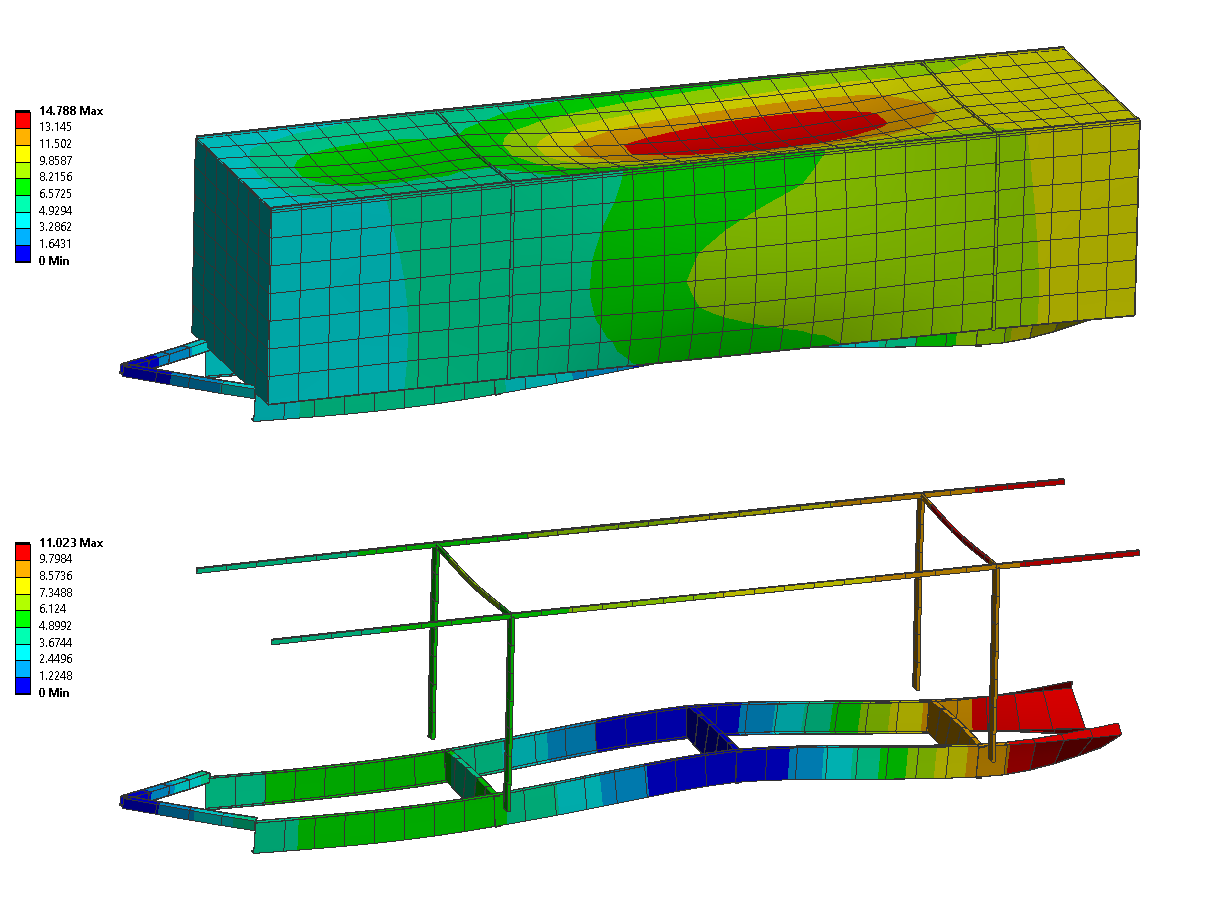
\includegraphics[width=1\linewidth]{04_figures/FEM 1.1.png}
  \caption{Deformation des Solar Butterflys im Lastfall der vertikalen Beschleunigung}
  \label{FEM 1.1}
\end{figure}

\subsubsection{Deformation - Lastfall 1.3 Longitudinale Beschleunigung}
\begin{figure}[H]
  \centering
  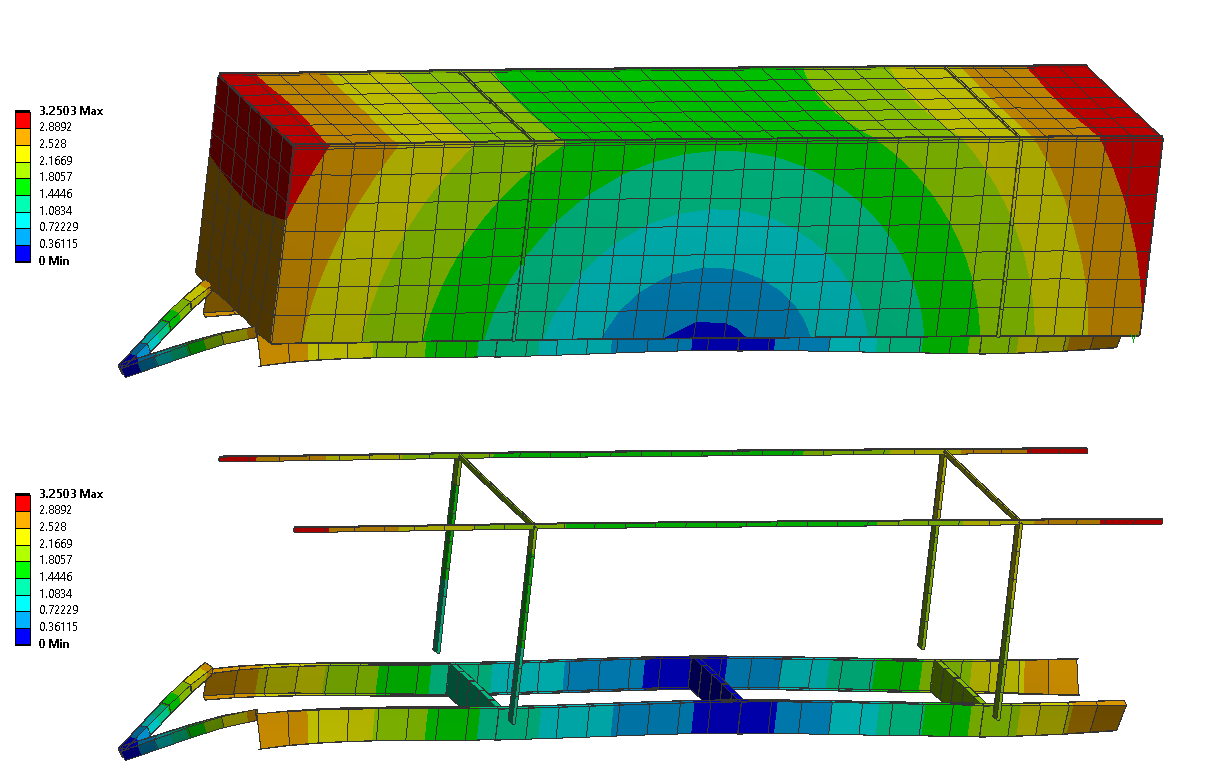
\includegraphics[width=1\linewidth]{04_figures/FEM 1.2.png}
  \caption{Deformation des Solar Butterflys im Lastfall der lateralen Beschleunigung}
  \label{FEM 1.3}
\end{figure}

\subsubsection{Deformation - Lastfall 1.4 Laterale Beschleunigung}
\begin{figure}[H]
  \centering
  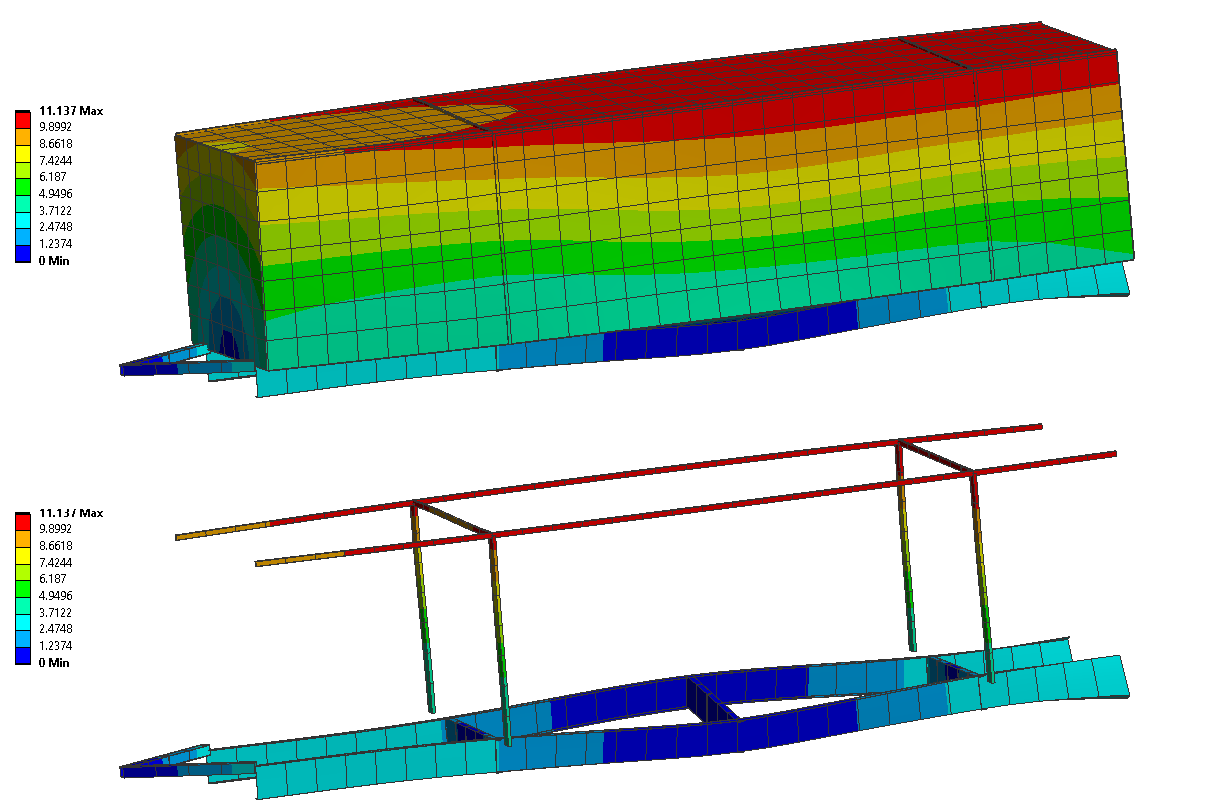
\includegraphics[width=1\linewidth]{04_figures/FEM 1.4.png}
  \caption{Deformation des Solar Butterflys im Lastfall der longitudinalen Beschleunigung}
  \label{FEM 1.4}
\end{figure}

\subsubsection{Deformation - Lastfall 1.5 Rotatorische Beschleunigung}
\begin{figure}[H]
  \centering
  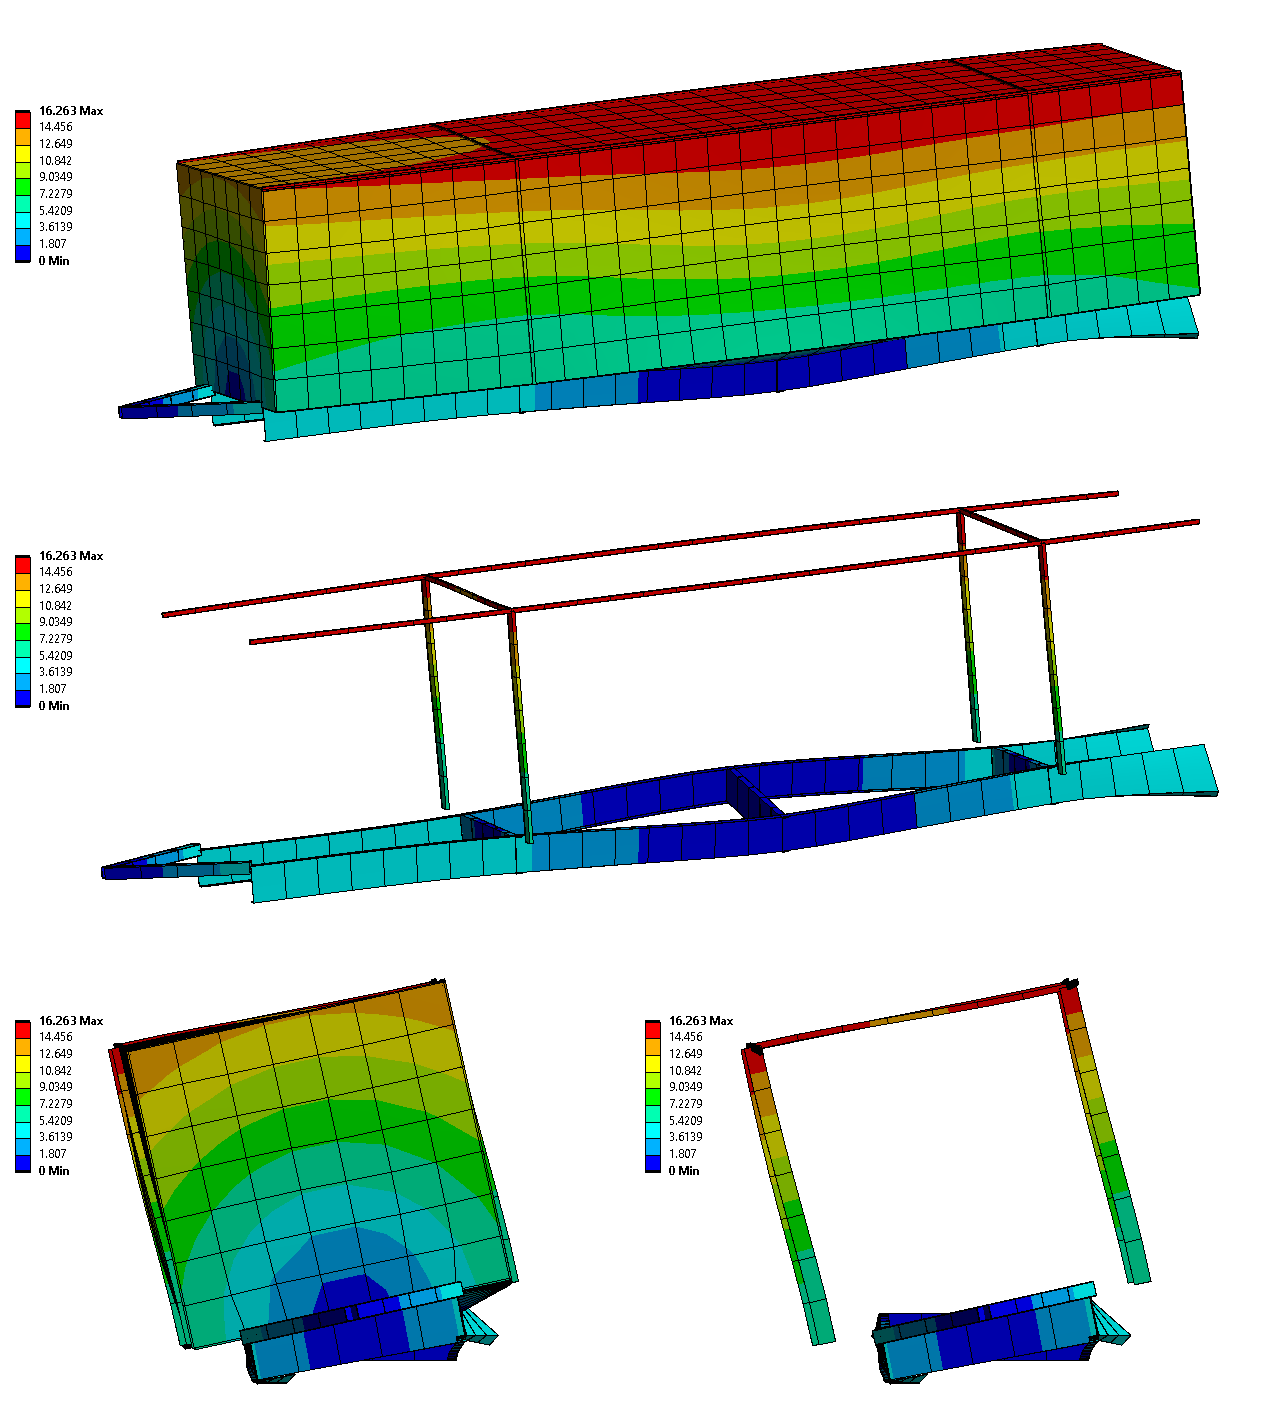
\includegraphics[width=1\linewidth]{04_figures/FEM 1.5.png}
  \caption{Deformation des Solar Butterflys im Lastfall der rotatorischen Beschleunigung}
  \label{FEM 1.5}
\end{figure}
\newpage

\end{document}
